\documentclass[12pt]{extarticle}

\usepackage{fancyhdr,amsfonts,graphicx,wrapfig,sidecap,float,adjustbox,subcaption,indentfirst,amsmath,hyperref}
\usepackage{listings}
\usepackage{color}
\usepackage{gensymb}

\usepackage[right=2.5cm,left=2.5cm,top=2.5cm,bottom=2.5cm]{geometry}

\pagestyle{fancy}
\lhead{Memorial University of Newfoundland}
\rhead{Department of Mathematics and Statistics}
\renewcommand{\headrulewidth}{0.4pt}

\lfoot{Mathematics 2130}
\cfoot{}
\rfoot{Fall 2015, Project 2}
\renewcommand{\footrulewidth}{0.4pt}
\flushbottom
\begin{document}
\begin{titlepage}
\vspace*{2in}
\begin{center}
{\LARGE Ancestry and Relations}
\end{center}

\vspace{2cm}

\abstract{In this paper, common trends amongst ancestry lines are analyzed and observed. The goal of the paper is to show how common ancestry forms in subsequent generations of offspring. The methods used include unique and non-unique testing. The affect of population growth on common ancestry is also observed using these methods. }


\vspace{3in}
\begin{flushright}
\begin{tabular}{l}
Project 3 \\
Mathematics 2130\\
Submitted by: John Hollett\\
Submitted to: Ivan Booth\\
\today
\end{tabular}
\end{flushright}


\end{titlepage}


\lhead{Ancestry and Relations}
\rhead{Math 2130}
\lfoot{John Hollett}
\rfoot{\thepage}
%\underheadoverfoot




\section{Introduction}
In this paper, how ancestry changes after each subsequent generation is discussed. Generations refers to individual sets of population. The tests range from basic conditions to more selective processes. These processes include random sampling with and without unique pairs. A pair refers to the duality between ancestors whether uniquely selected or not. 

In non-unique tests, the participants of each generation may be assigned the same parent. In unique testing, each participant contains two different parents. The difference between these tests will be explored and compared.

A program was written in C$^\#$ for tracing and tracking ancestry. This utility is required to perform the tests. The following equation describes the approximate number of generations required to see a common ancestor. This simple simulation is tasked with the responsibility of networking relationships in a decipherable manner. 
In the book by Richard Dawkins \cite{Ancestor}, equation (\ref{eqn}) was derived.

\begin{align}
\label{eqn}
C_{Generation} = \log_2 (N_{Population})
\end{align}
 
\section{Non-Unique Testing}
\subsection{Initial Test}
\begin{wrapfigure}[21]{l}{0.485\textwidth}
	\begin{center}
		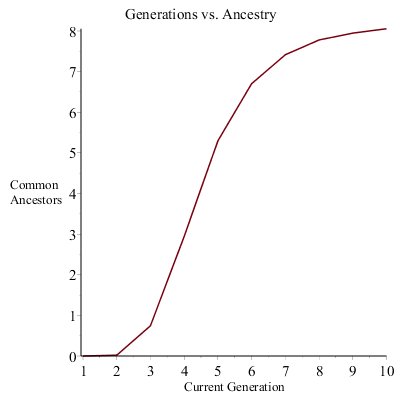
\includegraphics[scale=0.55]{Graph1.png}
		\caption{\small{Founding Population = 10, Generations = 10, Non-unique}}
		\label{fig:img1}
	\end{center}
\end{wrapfigure}
This section includes sampling and analysis of non-unique ancestors of varying sizes for each generation. The figure (\ref{fig:img1}) depicts the results of a test. An initial population of ten is selected, and a maximum of ten generations of humans. Each test is iterated 250 times.

In Figure (\ref{fig:img1}), the axes described is consistent with all figures in the paper. The information shown is the number of common ancestors for each generation starting from the founding generation. It serves as a proof in determining the program works correctly. A smaller size test was created and carried out to satisfy this requirement.
\begin{align}
\notag
C_{Generation} = \log_2(10) = 3.32
\end{align}
\indent With the data depicted by figure (\ref{fig:img1}), it is possible for one common ancestor to emerge after the second generation. Using equation (\ref{eqn}), the result supports the graph. It shows the utility created performs sufficiently to produce proper data.


\subsection{Further Testing}

\begin{figure}[h!]
	\caption{Non-unique Test}
	\begin{subfigure}{0.50\textwidth}
	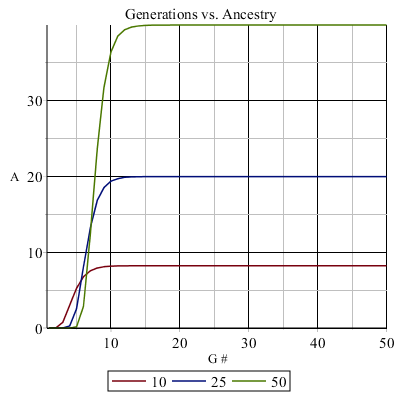
\includegraphics[scale=0.55]{Graph2.png}
	\caption{Test Pop 10, 25, 50}
	\label{fig:img2}
	\end{subfigure}
	\begin{subfigure}{0.50\textwidth}
	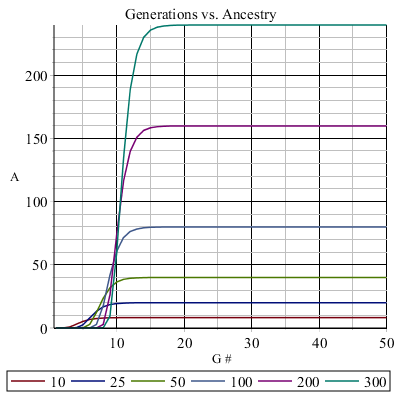
\includegraphics[scale=0.50]{Graph3.png}
	\caption{Test Pop 10, 25, 50, 100, 200, 300}
	\label{fig:img3}
	\end{subfigure}

\end{figure}

In this section, each test is compared using varying initial population sizes. The number of maximum generations remains constant at fifty. Based on Figure (\ref{fig:img2}), trends can be observed from the changing initial size. Each test show common ancestry emerges only after the third generation.

The tests using lower initial population show that the number of generations required to produce a non-changing common ancestor set changes from the initial population. This is also seen in larger founding population sizes. In Figure (\ref{fig:img3}), the data contradict perceived consistency in the number of generations required to observe a consistent ancestor set across all subsequent generations. Despite these results, the simulation returns the average number of generations it takes to form a common ancestry set for each founding population. 

The average of the number of ancestors carried through subsequent generations depicted in the figures (\ref{fig:img2}) and (\ref{fig:img3}) is roughly 80$\%$ of the starting population. Inversely, 20$\%$ of the founding population drops from the ancestry tree outright.  The data depicted in the next section addresses any influences uniquely selected ancestors exhibit.

\section{Unique Testing}


The data prepared in the previous section contrast the differences of unique and non-unique tests. Tests were re-ran for populations of $10, 25, 50$ and $100, 200, 300$. The number of maximum generations for which the tests were run remains fifty for this section. Figure (\ref{fig:img4}) and (\ref{fig:img5}) shows the average number of common ancestors in each generation. Using unique selection, the analysis reveals similar results. Checking the results with equation (\ref{eqn}) for each initial population supports figures (\ref{fig:img4}) and (\ref{fig:img5}).
\begin{figure}[h!]
	\caption{Unique and Non-Unique Analysis}
	\begin{subfigure}{0.50\textwidth}
		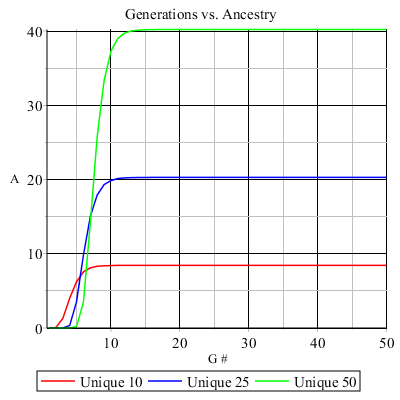
\includegraphics[scale=0.50]{Graph4.png}
		\caption{Unique}
		\label{fig:img4}
	\end{subfigure}
	\begin{subfigure}{0.50\textwidth}
		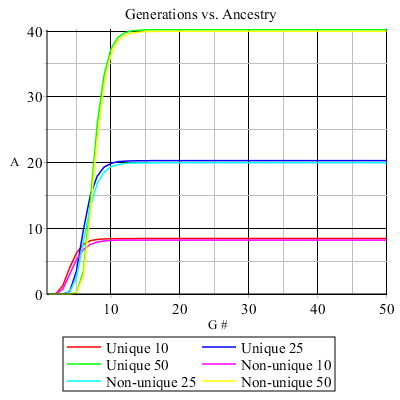
\includegraphics[scale=0.50]{Graph5.png}
		\caption{Unique and Non-unique}
		\label{fig:img5}
	\end{subfigure}
\end{figure}
\begin{wrapfigure}[17]{l}{0.475\textwidth}
	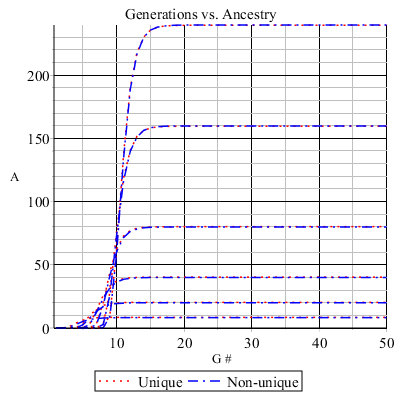
\includegraphics[scale=0.50]{Graph6.png}
	\caption{Unique vs. non-unique}
	\label{fig:img6}
\end{wrapfigure}
\begin{align}
\notag
C_{Generation} = \log_2(50) = 5.64
\end{align}

Figure (\ref{fig:img5}) depicts a unique ancestor set formed related to the founding size as seen in the previous section. This indicates that the difference between the two methods has negligible affect on the data.

Figure (\ref{fig:img6}) shows increasing initial populations. The increase in population in subsequent generations is a constant rate of $N$. The results of unique and non-unique tests show there is no significant difference between the two. The unique test results, on average, produce negligibly greater numbers of ancestors. Meanwhile the number of generations required to find an ancestor is greater although it is insignificant.

\section{Population Growth}

The tests carried out in this section simulates population growth. Growth is determined by a percentage that is constant amongst each generation. The population of any subsequent generation is determined by applying the percentage to the prior generation.
\begin{wrapfigure}[18]{l}{0.475\textwidth}
	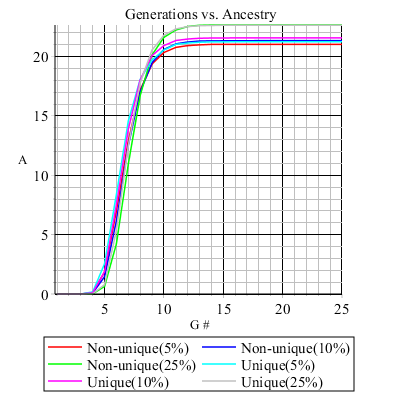
\includegraphics[scale=0.50]{Graph7.png}
	\caption{Pop Growth 5\%, 10\% ,25\%}
	\label{fig:img7}
\end{wrapfigure}
For the tests completed in this section, the populations will grow in size for each generation. The initial population for each test remains constant while the percentages of growth vary.

In figure (\ref{fig:img7}), despite population growth, the average number of ancestors remains relatively consistent in all tests. A significant difference is seen when the common ancestry set is found. 

With increasing population growth, the number of common ancestors increases. This result reflects the improved probability of selecting, and thus creating, more common ancestors from the founding set. 
\begin{align}
\notag
C_{\text{Generation}} = \log_2(25) = 4.64
\end{align}


The first common ancestor occurs at approximately the 5$^{\text{th}}$ generation. Following the 5$^{\text{th}}$ generation, the common ancestor set expands until the complete set is found. Using equation (\ref{eqn}), the result above agrees with figure (\ref{fig:img7}).

\section{Technical Details}

Explanation of the details of the testing methods is outlined in this section. The data collected were created using a simulation. The C$^\#$ programming language was used to create an iterative function to simulate data.

Two programmed objects named "Human" and "Generation" were used to correlate coherent data. A set of "Human" elements is stored in a generation. Previous sets are accessible in each "Generation", and the newly created "Generation" replaces the last as the current set. This is explained using sequences in mathematics . A sequence defined using the initial element $A_1$ and subsequent elements are described relative to the first in the sequence. The following example describes this process:

\begin{align}
\notag
& A_1 = \text{Generation}_0 \\
\notag
& A_N =\text{Generation}_{N-1}, \text{Where } N \geq 2 \\
\notag
&\text{Where Generation}_I \text{ is the population set at index I} 
\end{align}

A "Human" is defined as an object containing two ancestors. For subsequent generations, each "Human" contains ancestry inherited from its parents derived from the original population set. This process is described as:

\begin{align}
\notag
P &= \{p_0..p_N\}, \text{Where P denotes original ancestry set} \\
\notag
A &= \{a\in P | a_0,a_1, ..., a_N\} \\
\notag
B &= \{b\in P| b_0,b_1, ..., b_N\} \\
\notag
C &= A \cup B, \text{Where C is the ancestry set of the current Human} \\
\end{align}

Testing ancestry in the current generation, the simulation processes the elements in the set. Each "Human" and its ancestry set is intersected. If the result created is not an empty set, there is at least one common ancestor in the current generation.

New generations are created using parameters describing the number of new elements, previous generation and uniqueness. Creating a new population requires the prior generation. The two methods for creating each "Human" in the population is determined by reading the uniqueness parameter. A non-unique "Human" is created by selecting two random parents. Unique describes the same process as non-unique while requiring the parents to be unequal.
\begin{figure}[h!]
	\centering
	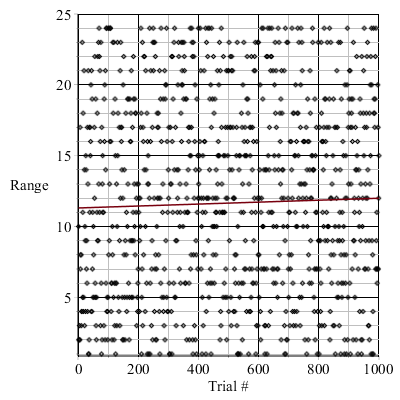
\includegraphics[scale=0.70]{RandomProof.png}
	\caption{Random Distribution}
	\label{fig:img8}
\end{figure}

Figure (\ref{fig:img8}) depicts the method used to randomly select a parent from a population of 25. While there is no definitive trend in this data, the line of best indicates gradual error. As the number of trials approaches completion, the trend line rests in the middle of the range. This suggests that most of the error is eliminated through increased testing. The error related to by the method used for selecting a parent is negligible but, other studies use more reliable methods. 

In a population set containing 25 elements, the randomly selected values lies between $0$ and $24$. The maximum value in figure (\ref{fig:img8}) is 24. A set of data containing 25 elements in the language chosen begins at 0 and ends at 24. The actual range is $0, ..., 24$ inclusive, resulting in 25 elements.

\section{Conclusion}

The tests performed in this paper show common ancestry occurs consistently after the number of generations found by equation (\ref{eqn}) . The figures show that the initial population affects presence of a common ancestor. Following the observation of a common ancestor, the figures depict consistently increasing traces of the founding members in each "Human".

In a paper on ancestry written by Douglas Rhode \cite{Population}, the results of tests were far more advanced and complex than those used in this test. The paper takes into account the various levels of segregation in the population, such as migration and life span.

While this paper does not detail such in depth analysis, real world application of the results does merit a meaningful conclusion. It provided evidence that common ancestry occurs and it should not surprise the reader that he/she may be distantly related to the writer and beyond.




\newpage

\lstset{basicstyle=\footnotesize,breaklines=true}
\lstset{framextopmargin=50pt,frame=bottomline}

\section{C$^{\#}$ Code}
\lstinputlisting[caption=Ancestry.cs]{Ancestry.cs}
\newpage
\begin{thebibliography}{99}
\bibitem{Ancestor}Dawkins, Richard. "The Ancestor's Tale". Houghton Mifflin, 2004, Print.
\bibitem{Population}"On the Common Ancestors of All Living Humans" \url{http://tedlab.mit.edu/~dr/Papers/Rohde-MRCA-two.pdf}, Douglas L. T. Rhode, Massachusetts Institute of Technology, 11 November 2003, Web 9 November 2015

\end{thebibliography}

\end{document}
